% Choose one to switch between slides and handout
%\documentclass[]{beamer}
\documentclass[handout]{beamer}

% Video Meta Data
\title{Bitcoin, Blockchain and Cryptoassets}
\subtitle{Transaction Consensus: Fork Theory}
\author{Prof. Dr. Fabian Schär}
\institute{University of Basel}

% Config File
% Packages
\usepackage[utf8]{inputenc} 
\usepackage{hyperref}
\usepackage{gitinfo2}
\usepackage{tikz}
\usepackage{amsmath}
\usepackage{bibentry}
\usepackage{xcolor}
\usepackage{caption}

% Beamer Template Options
\beamertemplatenavigationsymbolsempty
\setbeamertemplate{footline}[frame number]
\setbeamercolor{structure}{fg=black}
\setbeamercolor{footline}{fg=black}
\setbeamercolor{title}{fg=black}
\setbeamercolor{frametitle}{fg=black}
\setbeamercolor{item}{fg=black}
\setbeamercolor{}{fg=black}
\setbeamercolor{bibliography item}{fg=black}
\setbeamercolor*{bibliography entry title}{fg=black}
\setbeamertemplate{items}[square]
\setbeamertemplate{enumerate items}[default]
\captionsetup[figure]{labelfont={color=black},font={color=black}}
\captionsetup[table]{labelfont={color=black},font={color=black}}

\setbeamertemplate{bibliography item}{\insertbiblabel}

% Link Icon Command
\newcommand{\link}{%
    \tikz[x=1.2ex, y=1.2ex, baseline=-0.05ex]{% 
        \begin{scope}[x=1ex, y=1ex]
            \clip (-0.1,-0.1) 
                --++ (-0, 1.2) 
                --++ (0.6, 0) 
                --++ (0, -0.6) 
                --++ (0.6, 0) 
                --++ (0, -1);
            \path[draw, 
                line width = 0.5, 
                rounded corners=0.5] 
                (0,0) rectangle (1,1);
        \end{scope}
        \path[draw, line width = 0.5] (0.5, 0.5) 
            -- (1, 1);
        \path[draw, line width = 0.5] (0.6, 1) 
            -- (1, 1) -- (1, 0.6);
        }
    }

% Custom Titlepage
\defbeamertemplate*{title page}{customized}[1][]
{
  \vspace{-0cm}\hfill\includegraphics[width=2.5cm]{../config/logo_cif} 
  \includegraphics[width=1.9cm]{../config/seal_wwz} 
  \\ \vspace{2em}
  \usebeamerfont{title}\textbf{\inserttitle}\par
  \usebeamerfont{title}\usebeamercolor[fg]{title}\insertsubtitle\par  \vspace{1.5em}
  \small\usebeamerfont{author}\insertauthor\par
  \usebeamerfont{author}\insertinstitute\par \vspace{2em}
  \usebeamercolor[fg]{titlegraphic}\inserttitlegraphic
    \tiny \noindent \texttt{Commit Hash: \gitHash}\\ 
	\texttt{Commit Time: \gitAuthorIsoDate}\\ \vspace{1em}
  \link \href{https://github.com/cifunibas/Bitcoin-Blockchain-Cryptoassets/blob/main/slides/intro.pdf}
  {Get most recent version}\\
  \link \href{https://github.com/cifunibas/Bitcoin-Blockchain-Cryptoassets/blob/main/slides/intro.pdf}
  {Watch video lecture}\\ \vspace{1em}
  License: \texttt{Creative Commons Attribution-NonCommercial-ShareAlike 4.0 International}\\\vspace{2em}
  \includegraphics[width = 1.2cm]{../config/license}
}


%%%%%%%%%%%%%%%%%%%%%%%%%%%%%%%%%%%%%%%%%%%%%%
%%%%%%%%%%%%%%%%%%%%%%%%%%%%%%%%%%%%%%%%%%%%%%
\begin{document}

\thispagestyle{empty}
\begin{frame}[noframenumbering]
	\titlepage
\end{frame}

%%%

%%%
\begin{frame}{What is a Fork?}

\color{focus} Disagreement on the current state \color{black} of the ledger that, if persisting, leads to a \color{focus} split of the network \color{black}  into two or more competing database instances

\begin{columns}[T]
	\begin{column}{0.45\textwidth}
		\begin{figure}[h]
  			\center
  			\resizebox{0.9\textwidth}{!}{
			%%% Figure from: Schär, Fabian. "Blockchain Forks: A Formal Classification Framework and Persistency Analysis." (2020).

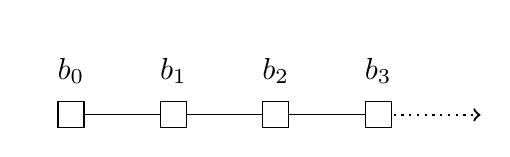
\begin{tikzpicture}[domain=1:10,scale=1.3, every node/.style={scale=1.1}]
\coordinate (o1) at (1,1);
\coordinate (o2) at (2,1);
\coordinate (o3) at (3,1);
\coordinate (o4) at (4,1);
\coordinate (o5) at (5,1);
\coordinate (o6) at (6,1);
\coordinate (o7) at (7,1);
\coordinate (o8) at (8,1);
\coordinate (o9) at (9,1);
\coordinate (o10) at (10,1);
\coordinate (n1) at (1,0.25);
\coordinate (n2) at (2,0.25);
\coordinate (n3) at (3,0.25);
\coordinate (n4) at (4,0.25);
\coordinate (n5) at (5,0.25);
\coordinate (n6) at (6,0.25);
\coordinate (n7) at (7,0.25);
\coordinate (n8) at (8,0.25);
\coordinate (n9) at (9,0.25);
\coordinate (n10) at (10,0.25);

  \draw[color=black] (o1) to[] (o2) to[] (o3) to[] (o4);
  \draw[color=black,thick, dotted, ->] (o4) to[] (o5);
  \node (rect) at (o1) [fill=white,draw,minimum width=0.3cm,minimum height=0.3cm] {};
  \node at (o1) [minimum width=1cm,minimum height=1cm,above] {${b}_0$};
  \node (rect) at (o2) [fill=white,draw,minimum width=0.3cm,minimum height=0.3cm] {};
  \node at (o2) [minimum width=1cm,minimum height=1cm,above] {${b}_1$};
  \node (rect) at (o3) [fill=white,draw,minimum width=0.3cm,minimum height=0.3cm] {};
  \node at (o3) [minimum width=1cm,minimum height=1cm,above] {${b}_2$};
  \node (rect) at (o4) [fill=white,draw,minimum width=0.3cm,minimum height=0.3cm] {};
  \node at (o4) [minimum width=1cm,minimum height=1cm,above] {${b}_3$};
\end{tikzpicture}

			}
		\end{figure}
	\end{column}
	\begin{column}{0.45\textwidth}
		\begin{figure}[h]
  			\center
  			\resizebox{0.9\textwidth}{!}{
			\input{../assets/figures/simple-fork.tex}
			}
		\end{figure}
	\end{column}
\end{columns}

\begin{columns}[T]
	\begin{column}{0.45\textwidth}
		\center		
		\footnotesize Simple Block Sequence
	\end{column}
	\begin{column}{0.45\textwidth}
		\center
 		\footnotesize Simple Fork 
	\end{column}
\end{columns}
\begin{center}
Figure: Illustration Blockchain Fork \cite{schar2020blockchain}
\end{center}

\uncover<2->{
\vspace{1em}	
$\Rightarrow$ Unique characteristic of Blockchains, not conclusively defined.
}

\end{frame}
%%%

%%%
\begin{frame}{Classification of Forks}

Placeholder: Missing Classification table 
	
\end{frame}
%%%	

%%%
\begin{frame}{Process-based Forks}

\textbf{Probabilistic block race:} Unintentionally coexisting consensus versions, caused by network propagation delays. 
\vspace{1em}	

\uncover<2->{
\textbf{Forced block race:} Deliberate mining of own chain with the goal to overtake consensus version.
\vspace{1em}	


\textbf{Block withholding:} Purposeful delay of propagation of own valid block candidate to gain head start on next block.
\vspace{1em}	
}

\uncover<3->{
$\Rightarrow$ All temporary and resolved through accumulated difficulty.
}
	
\end{frame}
%%%

%%%
\begin{frame}{Protocol-based forks}

\textbf{Client incompatibility:} Delta in consensus rule implementations by different network client software, causing some nodes to accept certain blocks rejected by others. Root causes:
\begin{itemize}
	\item Loosely defined consensus rules
	\item Software bugs
\end{itemize}
\vspace{0.5em}
Example: Upgrade to Bitcoin client 0.8 in 2013
\vspace{1em}	

\uncover<2->{
\textbf{Rule change:} Part of the network decides to alter the consensus rule set $S$ and proceed with adapted protocol.
\vspace{0.5em}

Example: Split of Bitcoin ABC over Blocksize increase.
\vspace{2em}	
	
}

\uncover<3->{
$\Rightarrow$ Not resolved automatically and may cause permanent splits.
}
	
\end{frame}
%%%

%%%
\begin{frame}{Types of Protocol-based Forks}


\begin{columns}[T]
	\begin{column}{0.3\textwidth}
		\center		
		\textbf{Soft Fork}\\
		\vspace{0.5em}
		\begin{figure}[h]
  			\resizebox{0.9\textwidth}{!}{
			%%% Figure from: Schär, Fabian. "Blockchain Forks: A Formal Classification Framework and Persistency Analysis." (2020).

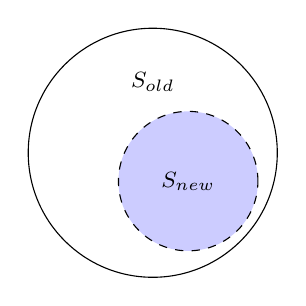
\begin{tikzpicture}[domain=0:8,scale=0.9, every node/.style={scale=1}]
  \filldraw[draw=black,fill=white] (0,0) circle (50pt) node[below=-1.15cm,color=black]{\footnotesize{$S_{old}$}};
  \filldraw[draw=black,fill=blue!20,dashed] (0.5,-0.4) circle (28pt) node[color=black]{\footnotesize{$S_{new}$}};
\end{tikzpicture}

			}
		\end{figure}
		\vspace{1em}
		$S_{new}\subset S_{old}$
	\end{column}
	\begin{column}{0.3\textwidth}
		\center
 		\textbf{Hard Fork}\\
 		\vspace{1em}
 		\begin{figure}[h]
  			\center
  			\resizebox{0.9\textwidth}{!}{
			\input{../assets/figures/hard-fork.tex}
			}
		\end{figure}
 		\vspace{1.5em}
 		$S_{new}\supset S_{old}$
	\end{column}
		\begin{column}{0.3\textwidth}
		\center
 		\textbf{Forced Fork}\\
 		\vspace{0.5em}
 		\begin{figure}[h]
  			\center
  			\resizebox{0.9\textwidth}{!}{
			%%% Figure from: Schär, Fabian. "Blockchain Forks: A Formal Classification Framework and Persistency Analysis." (2020).

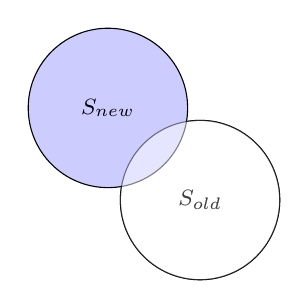
\begin{tikzpicture}[domain=0:8,scale=0.9, every node/.style={scale=1}]
  \filldraw[draw=black, fill=white] (0.9,-0.9) circle (32pt) node[color=black]{\footnotesize{$S_{old}$}};
  \filldraw[draw=black,fill=blue!20] (-0.4,0.4) circle (32pt) node[color=black]{\footnotesize{$S_{new}$}};
  \filldraw[draw=black, fill=white, opacity=0.5] (0.9,-0.9) circle (32pt) node[color=black]{\footnotesize{$S_{old}$}};
\end{tikzpicture}

			}
		\end{figure}
		\vspace{0.8em}
 		$(S_{new}\setminus S_{old} \neq \emptyset)$\\$\wedge$\\ $(S_{old}\setminus S_{new} \neq \emptyset)$
	\end{column}
\end{columns}

\vspace{0.5em}

\begin{center}
	Figure: Types of protocol-based forks \cite{schar2020blockchain}
\end{center}

	
\end{frame}
%%%

%%%
\begin{frame}{Fork Persistency by Type and Dominance Scenario}

\center \footnotesize
$P(\,b \in S_{new} \wedge b \in S_{old})\, = \dfrac{r_{old}}{R} \left( 1-\frac{|S_{new} \cap S_{old}|}{|S_{old}|}\right) + \dfrac{r_{new}}{R} \left( 1-\frac{|S_{new} \cap S_{old}|}{|S_{new}|}\right)$ 
\label{eq:forkprobability}

\vspace{1.5em}


	\begin{table}
		\input{../assets/figures/fork-types.tex}
		\caption{Persistency by fork type and scenario \cite{schar2020blockchain}}
		\label{tbl:forkpersistencies}
	\end{table}

	


	
\end{frame}
%%%



%%%
\begin{frame}{Why Care about Forks?}

\textbf{Uncertainty:} Confirmation status of transactions.
\vspace{1.5em}

\textbf{Confusion:} Which one is the "main" version.
\vspace{1.5em}

\textbf{Undermining trust:} Case of digital assets.
\vspace{1.5em}

\textbf{Cost driver:} Maintaining compatibility.
\vspace{1.5em}

\color{focus} \textbf{But:} \color{black} Pillar for political freedom and resilience against arbitrary changes.

	
\end{frame}
%%%	

%%%
\begin{frame}%[allowframebreaks]
\frametitle{References and Recommended Reading}

	\bibliographystyle{amsplain}
	\bibliography{../assets/bib/refs}

\end{frame}


\end{document}